\documentclass{article}
\usepackage[T1]{fontenc}
\usepackage{color}
\usepackage{cite}
\usepackage[pdftex, bookmarks=true]{hyperref}
\usepackage{amsmath}
\usepackage{listings}
\usepackage{tikz}
\usepackage{pgfplots}

% Make a draft watermark.
% \usepackage{draftwatermark}
% \SetWatermarkFontSize{40pt}
% \SetWatermarkScale{4.0}

% TODO: Use bibtex or some better bibliography management
% tool.



% Define the speculative C++1y language.
\lstdefinelanguage{C++1y}{alsolanguage=C++,
                          escapechar=@,
                          breakatwhitespace=true,
                          morekeywords = {alignof, 
                                          decltype, 
                                          concept, 
                                          axiom, 
                                          requires, 
                                          property}}

% Program output
\lstdefinelanguage{Output}{}

% EBNF
\lstdefinelanguage{Ebnf}
{
  escapechar=@,
  basicstyle=\itshape\small
}


% Default formatting for listings.
%
% TODO: Define this as a style and make the code and program macros refer
% to the style.
\lstset{language=C++1y,
        basicstyle=\ttfamily\small,
        keywordstyle=\bfseries\color[rgb]{0,0,1},
        stringstyle=,
        xleftmargin=1em,
        showstringspaces=false,
        commentstyle=\rmfamily\itshape,
        columns=flexible,
        keepspaces=true,
        texcl=true}




% Define formatting for code.
\newcommand{\code}[1]{\lstinline @#1@}

% Define an environment for C++ programs.
\lstnewenvironment{program}{\lstset{language=C++1y}}{}

% Define an environment for program output.
\lstnewenvironment{progout}{\lstset{language=Output}}{}

% Define an environment for EBNF Grammars
\lstnewenvironment{ebnf}{\lstset{language=Ebnf}}{}

% Define formatting for indented blocks of text
\newcommand{\blockindent}[1]{\hangindent=#1\setlength{\parindent}{#1}\setlength{\parskip}{1em plus0.2em minus0.2em}}

% Define formatting for indented blocks of text
\newcommand{\blockunindent}{\hangindent=0em\setlength{\parindent}{0em}\setlength{\parskip}{0em}}


\begin{document}

\noindent\textbf{Document Number:} D0429R0\\
\textbf{Date:} 2016-08-31\\
\textbf{Reply to:} whatwasthataddress@gmail.com\\
\textbf{Audience:} LWG/LEWG

\title{\textbf{\Large A Standard \code{flat_map}}}
\author{
  \makebox[.25\linewidth]{T. Zachary Laine}\\NVIDIA\\
}
\date{}
{\let\newpage\relax\maketitle}


\section{Introduction}

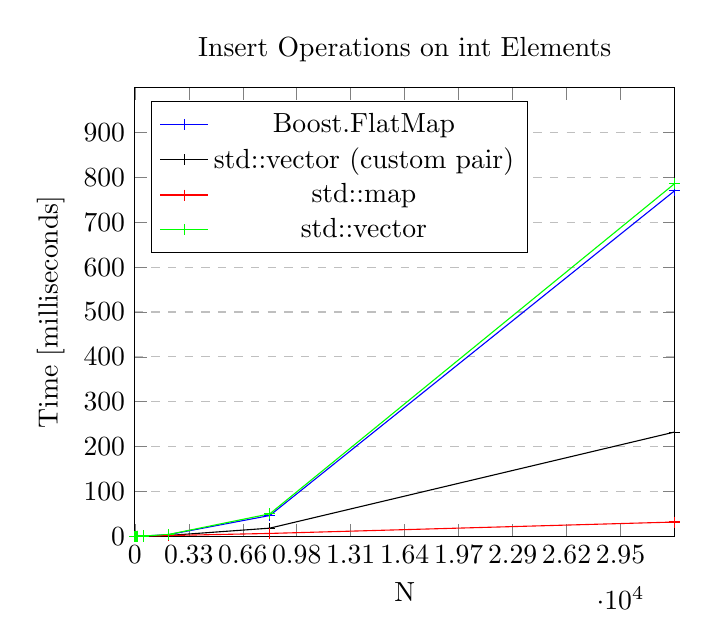
\begin{tikzpicture}
    \begin{axis}[
        title={Insert Operations on int Elements},
        xlabel={N},
        ylabel={Time [milliseconds]},
        xmin=0, xmax=32768.0,
        ymin=0, ymax=1000.0,
        xtick={0.0,3276.8,6553.6,9830.4,13107.2,16384.0,19660.8,22937.6,26214.4,29491.2},
        ytick={0.0,100.0,200.0,300.0,400.0,500.0,600.0,700.0,800.0,900.0},
        legend pos=north west,
        ymajorgrids=true,
        grid style=dashed,
        legend entries={Boost.FlatMap,std::vector (custom pair),std::map,std::vector}
        ]

    \addplot[color=blue,mark=+,]
        coordinates {(8,0.0061)(32,0.009)(128,0.0466)(512,0.3269)(2048,3.4296)(8192,46.1462)(32768,770.289)};

    \addplot[color=black,mark=+,]
        coordinates {(8,0.0051)(32,0.0133)(128,0.1292)(512,0.2641)(2048,1.6346)(8192,17.9527)(32768,232.288)};

    \addplot[color=red,mark=+,]
        coordinates {(8,0.0084)(32,0.0187)(128,0.0794)(512,0.3573)(2048,1.4816)(8192,6.1507)(32768,31.5773)};

    \addplot[color=green,mark=+,]
        coordinates {(8,0.0045)(32,0.0135)(128,0.0535)(512,0.3669)(2048,3.8914)(8192,49.8729)(32768,786.225)};

    \end{axis}
\end{tikzpicture}


\label{sec:intro}

This paper outlines what a (mostly) API-compatible, non-node-based \code{map}
might look like.  Rather than presenting a final design, this paper is
intended as a starting point for discussion and as a basis for future work.
Specifically, there is no mention of \code{multimap}, \code{set}, or
\code{multiset}.  Those will be added in later papers.

\section{Motivation and Scope}

There has been a strong desire for a more space- and/or runtime-efficient
representation for \code{std::map} among C++ users for some time now.  This
has motivated discussions among the members of SG14, numerous articles and
talks, and an implementation in Boost, \code{boost::container::flat_map}.
Virtually everyone who makes games, low-level, or embedded-system software
in C++ uses the Boost implementation, or one that they rolled themselves.

\section{Impact on the Standard}

This proposal is a pure extension.  It has no impact on the existing standard.

\section{Proposed Design}

\subsection{Design Goals}

The Boost.Container documentation gives a nice summary of the tradeoffs
between node-based and flat associative containers (quoted here, mostly
verbatim).  Note that they are not purely positive:

\begin{itemize}
  \item Faster lookup than standard associative containers.

  \item Much faster iteration than standard associative
    containers.

  \item Random-access iterators instead of bidirectional iterators.

  \item Less memory consumption for each element.

  \item Improved cache performance (data is stored in contiguous memory).

  \item Non-stable iterators (iterators are invalidated when inserting and
    erasing elements).

  \item Non-copyable and non-movable values types can't be stored.

  \item Weaker exception safety than standard associative containers
    (copy/move constructors can throw when shifting values in erasures and
    insertions).

  \item Slower insertion and erasure than standard associative containers
    (specially for non-movable types).
\end{itemize}

The overarching goal of this proposal is to define a \code{flat_map} for
standardization that fits the above gross profile, while leaving maximum room
for customization by users.

\subsection{Design}

\subsubsection{\code{flat_map} Is a Container Adapter}

\code{flat_map} is an adapter for an underlying storage type.  This storage
type is configurable via the template parameter \code{Container}.
\code{Container} must be a \textit{contiguous container} (\S23.2.1/13).
\code{vector} is a great candidate for this, but limiting \code{flat_map} only
to use \code{vector} for its storage would be a mistake.  Many other suitable
replacements exist, each suited to a certain use.  A user may have a
small-buffer implementation of \code{vector}, like LLVM's \code{SmallVector},
or \code{boost::container::small_vector}.  The user may also want to avoid
allocations altogether, if the maximum number of elements N is know \textit{a
  priori}.  If so, \code{boost::container::static_vector} could be used.

\subsubsection{Interface Differences From \code{map}}

\begin{itemize}
  \item Members \code{capacity()}, \code{reserve()}, and \code{shrik_to_fit()}
    have been added, with the same semantics as the corresponding members of
    \code{vector}.

  \item Several new constructors have been added that take objects of the
    \code{Container} type.  These members must only be used if the given
    container is already sorted.

  \item The \code{extract()} overloads from \code{map} are replaced with
    \code{Container extract()}, that moves out the entire storage of the
    \code{flat_map}.  Similarly, the \code{insert()} members taking a node
    have been replaced with a member \code{void replace(Container&&)}, that
    moves in the entire storage.

    Many users have noted that M insertions of elements into a map of size N
    is O(M$\cdot$log(N+M)), and when M is known it should be possible instead
    to append M times, and then re-sort, as one might with a sorted
    \code{vector}.  This makes the insertion of multiple elements closer to
    O(N), depending on the implementation of \code{sort()}.

    Such users have often asked for an API in
    \code{boost::container::flat_map} that allows this pattern of use.  Other
    flat-map implementations have undoubtedly added such an API.  The
    extract/replace API instead allows the same optimization opportunities
    without violating the class invariants.

  \item Several new constructors and an \code{insert()} overload use a new tag
    type, \code{ordered_unique_sequence_tag}.  These members must only be used
    if the given sequence is already sorted.  This can allow much more
    efficient construction and insertion.
\end{itemize}

\subsubsection{\code{flat_map} Requirements}

(TODO! Change the synopsis to reflect this!) Since the underlying container is
contiguous and elements may be moved or copied during inserts and erases, the
element type of \code{Container} must be \code{pair<Key, T>}, not
\code{pair<const Key, T>}.  Even so, the element type of \code{flat_map}
should still be \code{pair<const Key, T>}, for drop-in compatibility with
\code{map} (\S23.2.4/5).

Only the underlying container is allocator-aware.  \S23.2.4/7 regarding
allocator awareness does not apply to \code{flat_map}.

Validity of iterators is not preserved when mutating the underlying container
(i.e. \S23.2.4/9 does not apply).

The exception safety guarantees for associative containers (\S23.2.4.1) do not
apply.

The rest of the requirements follow the ones in (\S23.2.4 Associative
containers), except \S23.2.4/10, which applies to members not in
\code{flat_map} and select portions of the table in \S23.2.4/8.  These table
differences are outlined in ``Member Semantics'' below.

\subsubsection{\code{Container} Requirements}

Any contiguous container supporting operations \code{capacity()},
\code{reserve()}, and \code{shrik_to_fit()} can be used for the
\code{Container} template parameter.  \code{Container} must have a
\code{value_type} of \code{pair<Key, T>}.

\subsubsection{Member Semantics}

Members \code{capacity()}, \code{reserve()}, and \code{shrik_to_fit()} have
the same semantics as the corresponding members of \code{vector}.

Each member taking a \code{Container} reference or taking a parameter of type
\code{ordered_unique_sequence_tag} has the precondition that the given
elements are already sorted by \code{Compare}, and that the elements are
unique.

Each member taking an \code{Alloc} template parameter only participates in
overload resolution if \code{uses_allocator_v<Container, Alloc>} is
\code{true}.

Other member semantics are the same as for \code{map}.

\subsubsection{\code{flat_map} Synopsis}

\lstinputlisting[language=C++]{map_synopsis.hpp}


\end{document}
